\documentclass{article}
%\usepackage{fullpage}
\usepackage{sidecap}
\usepackage{mdframed}
\usepackage{mathtools}
\usepackage{mhchem}
\usepackage{amssymb}
\usepackage{amsmath}
\usepackage{bm}
\usepackage{gensymb}
\usepackage{siunitx}
\usepackage{cancel}
\usepackage{graphicx}
\usepackage{subcaption}
\usepackage{hyperref}
\author{Mann, J}
\title{Day 2 Notes}
\date{September 15, 2015}
\newenvironment{aside}{\begin{mdframed}}{\end{mdframed}}
\renewcommand{\d}[0]{\mathrm{d}}
\newcommand{\note}[1]{\\\\\textit{\textbf{Note: }}#1\\\\}
\newcommand{\pOne}[2]{\frac{\partial #1}{\partial #2}}
\renewcommand{\deg}[0]{\degree}
\newcommand{\pTwo}[2]{\frac{\partial^2 #1}{\partial #2^2}}
\newcommand{\dOne}[2]{\frac{\d #1}{\d #2}}
\newcommand{\dTwo}[2]{\frac{\d^2 #1}{\d #2^2}}
\newcommand{\diag}[1]{\bcancel{#1}}
\newcommand{\matr}[1]{\bm{#1}}
\graphicspath{{Day6NotesPics/}}
\begin{document}
\maketitle{}
\begin{section}{Introduction}
  Tensor analysis is designed to make it so that you don't have to worry about the coordinate system until you actually do a calculation.

	Example: 

	\begin{align*}
		\vec{F} = m\vec{a}
	\end{align*}
	which is independent of coordinates.

	A moment to explain Covariant/contravariant tensors in practice:

	Example: Let us define a function $f(\vec{x})$:
\begin{align*}
	f(\vec{x}) = a_1 x_1 + a_2 x_2 + \dots + a_n x_n\\
	f(\vec{x}) = \begin{bmatrix}a_1 & a_2 & \dots & a_n\end{bmatrix} \begin{bmatrix}x_1 \\ x_2 \\ \vdots \\ x_n\end{bmatrix}
\end{align*}
Where $a_i$ is a constant, and $x_i$ is a variable representing position.  $\vec{a}$ is covariant, while $\vec{x}$ is contravariant.

Another notation is:
\begin{align*}
	a[\vec{x}] = f(\vec{x})
\end{align*}<++>

	$\vec{F}$ and $\vec{a}$ are \underline{vectors}, which are Rank 1 contravariant tensors. In \href{https://en.wikipedia.org/wiki/Einstein_notation#Vector_representations}{(Einstein)} index notation, 
  \begin{align*}
    F^i = m a^i\\
    \d x^i = v^i \d t\\
    \d v^i = a^i \d t
  \end{align*}
	\note{Upper index is for contravariant tensors}

  Rank must be conserved, just like dimensional analysis units must be conserved.
  
	Let $\phi(x)$ be a scalar function, which is a Rank 0 contravariant tensor. Then
	$$-\pOne{\phi(\underline{x})}{x^i} = F_i$$ is a covariant tensor of rank 1.


\end{section}
\begin{section}{Covariant and Contravariant Tensors}
  Transformations:
	\begin{figure}[h]
		\centering
		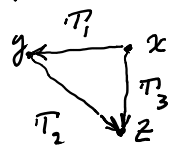
\includegraphics[height=060pt]{Transformation1}
		\caption{Transformation $T_3$ is the composition of transformations $T_1$ and $T_2$}
		\label{fig:T1}
	\end{figure}
	\begin{align*}T_1 := \begin{cases}y^i = y^i(x^1,x^2,x^3)\end{cases}\\
  T_2 :=\begin{cases} z^i = z^i(y^1,y^2,y^3)\end{cases}\\
    \end{align*}
    Now think of a composite function $\circ$, (like multiplication, addition, etc of $\mathbb{R})$
    \begin{aside}
			For example, if we were dealing with scalars, $A\circ B$ could be $A\times B$, $A+B$, or $A\div B$.

			$\circ$ needs to be Associative ($T_4\circ(T_2\circ T_1) = (T_4\circ T_2) \circ T_1$
			
			The point you need to get to is that $T_1,T_2,$ etc. form a group
		\end{aside}
      \begin{align*}
      T_2 &\circ T_1 := \begin{cases}z^i = z^i(y^i(x))\end{cases}\\
	T_2&\circ T_1 = T_3
      \end{align*}
      \begin{align*}
	T_4\circ (T_2\circ T_1) = (T_4\circ T_2)\circ T_1\\
	1 + (2+3) = (1+2) + 3
      \end{align*}

      There are coordinate systems so that I can 
      \begin{align*}
	T_i\circ T_j = T_3 \text{for all well posed coordinate systems}
      \end{align*}

      Continuity condition $y^i = y^i(x) - C^1$ 1st derivatives also continuous

      \begin{align*}
	\d T = \begin{pmatrix}
	  \pOne{y^1}{x^1} & \pOne{y^1}{x^2} & \pOne{y^1}{x^3}\\ 
	  \pOne{y^2}{x^1} & \pOne{y^2}{x^2} & \pOne{y^2}{x^3}\\ 
	  \pOne{y^3}{x^1} & \pOne{y^3}{x^2} & \pOne{y^3}{x^3}
	\end{pmatrix}
      \end{align*}
      The determinant of $\d T$ is called the jacobian $J(T)\neq 0$, this also implies that the inverso of $T,T^{-1}$ also exists. 
      \begin{align*}
	T\circ T^{-1} = T^{-1}\circ T = I
      \end{align*}
      $I := y^i = x^i$

      Exsitence of ${T}$, Definition of $\circ$, I have $J\neq 0$, identity, inverse - This system is a group GROUP.
      \begin{subsection}{Example of the Jacobian being 0}
	PICTURE
	Example: The convesion between cartesian and spherical coordinates. At a finite number of points, the Jacobian will be equal to zero. (R=0)
	The GROUP here includes the transformation between cartesian and spherical coordinates, as well as every other transformation you could make.
      \end{subsection}
    \end{section}
      \begin{section}{Consider}
				\begin{align*}y^i = y^i(\underline{x})\\
	  \d y^i = \pOne{Y^i}{x^j} \partial x^j
	\end{align*}

	Using the Einstein sum convention $A_{kl}^i$ suppose $A_{il}^i \equiv \sum_{i=1}^{3}A_{il}^i$
	\note{$\d y^i$ is a contravariant Rank 1 tensor transformed from $\d x^j$ through the matrix $\pOne{y^i}{x^j}$}
	\begin{align*}
		\text{The }y^i\text{ coordinate system} &\leftarrow  \text{the }x^i\text{ coordinate system}\\
		A^i  &\leftarrow \pOne{y^i}{x^i}A^j
	\end{align*}

	  \begin{align*}
			\pOne{\phi}{x^i}\pOne{x^i}{y^j} =\pOne{\phi}{y^j}\text{ a \underline{covariant} vector}
	  \end{align*}
	\end{section}
	  \begin{section}{Matrices}
	    \newcommand{\eOne}[0]{\vec{e}_1}
	    \newcommand{\eTwo}[0]{\vec{e}_2}
	    \newcommand{\eThree}[0]{\vec{e}_3}
	    \newcommand{\ei}[0]{\vec{e}_i}
	    \newcommand{\ej}[0]{\vec{e}_j}
			Let us define variables
			\begin{align*}
			\vec{e}_1, \vec{e}_2, \vec{e}_3\\
			\eOne \rightarrow \pOne{y^i}{x^1}, \text{etc.}
			\end{align*}
			and 
			\begin{align*}
				g_{ij} = \ei\cdot \ej
			\end{align*}
			Which is to say that $\matr{g}$ is a metric tensor.

			Now, let us look at derivatives:
	$$\d S^i = \begin{pmatrix}\d x^1 & \d x^2 & \d x^3\end{pmatrix}\begin{pmatrix}\d x^1 \\ \d x^2 \\ \d x^3\end{pmatrix} = (\d x)^t \d x$$
	in cartesian coordinates.  
	\begin{align*}
		\d x^i &= \pOne{x^i}{y^j} \partial y^j
	\end{align*}
	Gone from \begin{align*}
	    dS^2 &= (\d x^1)^2 + (dx^2)^2 + (dx^3)^2\\
			\delta_{ij} &= \begin{cases}1 \text{ if } i=j\\
																 0 \text{ if } i\neq j\end{cases}\\
	  \d S^2 &= \delta_{ij}\d x^i dx^j\\
	  \d S^2 &= g_{ij}\d x^i \d x^j\\
	  J &= \sqrt{g}\\
		g &= \det{(\matr{g})}
	\end{align*}
	Now that we have $g_{ij}$ defined, does there exist $g^{kl}$ such that 
	\begin{align*}
		g_{ij}g^{jl} = \delta_i^l = \begin{cases}1\text{ if }i=l\\ 0\text{ if }i\neq l\end{cases}?
	\end{align*}
	 It turns out that $g^{kl}$ is the matrix inverse of $g_{ij}$

	 \begin{align*}
		 A^i &= \text{contravariant}\\
		 A^ig_{ij} &= A_j\\
		 A_j g^{ij} &= A^i
	 \end{align*}

	 $\pOne{\phi}{x^i} g^{ij} = \left(\pOne{\phi}{x^i}\right)_\text{contravariant}^j | B_i g^{ij} = B^j$
	 \note{\begin{align*}\vec{F} = m\vec{a} + -\nabla \phi\end{align*}
	$\vec{a}$ is contravariant, $-\nabla\phi$ is covariant, so we need to rewrite this.
	\begin{align*}
		F^i = ma^i - \pOne{\phi}{x^j}g^{ji}
	\end{align*}
Now this is tensor consistent, both sides of the ``$=$'' are contravariant.}

	Now, the sort of tensors we use in this course, we don't have to worry about the coordinate system that we're in. A place where you have to be very careful is when the surface is curved. For formulating mass/momentum transport to deal with interfaces, we can deal with just cartesian tensors.



\end{section}
\begin{section}{Experimental Methods}
  Define surface tension as a function of $T,P,c,$ etc.
  \begin{enumerate}
    \item Geometric Methods
      \begin{itemize}
	\item Capillary Rise (since the 1700's!) Take a glass tube with a small inside diameter, put it into your solution, and you will get liquid that rises up to a head height. That is related to the surface tension.
      \end{itemize}
    \item Force Methods
  \end{enumerate}
\end{section}
\end{document}
